%% Version 5.0, 2 January 2020
%
%%%%%%%%%%%%%%%%%%%%%%%%%%%%%%%%%%%%%%%%%%%%%%%%%%%%%%%%%%%%%%%%%%%%%%
% TemplateV5.tex --  LaTeX-based template for submissions to the
% American Meteorological Society
%
%%%%%%%%%%%%%%%%%%%%%%%%%%%%%%%%%%%%%%%%%%%%%%%%%%%%%%%%%%%%%%%%%%%%%
% PREAMBLE
%%%%%%%%%%%%%%%%%%%%%%%%%%%%%%%%%%%%%%%%%%%%%%%%%%%%%%%%%%%%%%%%%%%%%

%% Start with one of the following:
% DOUBLE-SPACED VERSION FOR SUBMISSION TO THE AMS
\documentclass[twocol]{ametsocV5}


% TWO-COLUMN JOURNAL PAGE LAYOUT---FOR AUTHOR USE ONLY
% \documentclass[twocol]{ametsocV5}


% Enter packages here. If too many math alphabets are used,
% remove unnecessary packages or define hmmax and bmmax as necessary.

\newcommand{\hmmax}{0}
\newcommand{\bmmax}{0}
\usepackage{amsmath,amsfonts,amssymb,bm}
\usepackage{mathptmx}%{times}
\usepackage{newtxtext}
\usepackage{newtxmath}


%%%%%%%%%%%%%%%%%%%%%%%%%%%%%%%%

%%% To be entered by author:

%% May use \\ to break lines in title:

\title{Title here}


\authors{Elio Campitelli
\correspondingauthor{Elio Campitelli,elio.campitelli@cima.fcen.uba.ar}
and Leandro Díaz
}

\affiliation{CIMA UBA blablabla}

\extraauthor{Carolina Vera
}


%%%%%%%%%%%%%%%%%%%%%%%%%%%%%%%%%%%%%%%%%%%%%%%%%%%%%%%%%%%%%%%%%%%%%
% ABSTRACT
%
% Enter your abstract here
% Abstracts should not exceed 250 words in length!
%


\abstract{Enter the text of your abstract here. This is a sample American
Meteorological Society (AMS) \LaTeX~template. This document provides
authors with instructions on the use of the AMS \LaTeX~template. Authors
should refer to the file amspaper.tex to review the actual \LaTeX~code
used to create this document. The template.tex file should be modified
by authors for their own manuscript.}

\begin{document}

%% Necessary!
\maketitle

\bibliographystyle{ametsoc2014}
%%%%%%%%%%%%%%%%%%%%%%%%%%%%%%%%%%%%%%%%%%%%%%%%%%%%%%%%%%%%%%%%%%%%%
% SIGNIFICANCE STATEMENT/CAPSULE SUMMARY
%%%%%%%%%%%%%%%%%%%%%%%%%%%%%%%%%%%%%%%%%%%%%%%%%%%%%%%%%%%%%%%%%%%%%
%
% If you are including an optional significance statement for a journal article or a required capsule summary for BAMS
% (see www.ametsoc.org/ams/index.cfm/publications/authors/journal-and-bams-authors/formatting-and-manuscript-components for details),
% please apply the necessary command as shown below:
%
\statement
This is significant becasue\ldots{}



%%%%%%%%%%%%%%%%%%%%%%%%%%%%%%%%%%%%%%%%%%%%%%%%%%%%%%%%%%%%%%%%%%%%%
% MAIN BODY OF PAPER
%%%%%%%%%%%%%%%%%%%%%%%%%%%%%%%%%%%%%%%%%%%%%%%%%%%%%%%%%%%%%%%%%%%%%
%

\section{Introduction}

blabalblba introdocction. SAM\ldots{} yada yada circulation.. Lorem
ipsum dolor sit amet, hac curae turpis sollicitudin vulputate quisque
sapien nullam curae integer. Torquent porttitor et et vulputate blandit
velit sed sed at velit eget arcu. Senectus, taciti justo eu sem purus
vestibulum pellentesque quis ac. Ac facilisi, amet consectetur mauris
fringilla sit. Est fusce, augue orci dictumst lacinia et elementum
dapibus orci eu, luctus ut luctus. Phasellus magna ut felis vitae metus
non non. In maecenas taciti. Hendrerit bibendum placerat. Molestie est
enim ante amet natoque consequat hendrerit, pharetra ridiculus.
Ultricies mauris donec leo eu, parturient praesent. Ridiculus sociis
ligula, ultricies augue, sagittis, turpis et. A netus at sagittis enim
nisl aliquet sed.

Justo id ut dolor faucibus ac justo orci volutpat vivamus nisl. Eu
sollicitudin, semper sed vitae et praesent vitae diam venenatis. Felis
vitae, velit risus id donec et. Neque nec id. Tellus nisl, vivamus sed
faucibus, non, per scelerisque ac arcu eget mus himenaeos imperdiet.
Purus eu quis felis mauris, ultricies et luctus integer orci. Lobortis
eget nec cras egestas feugiat. At mattis eget mus aliquam pellentesque
mauris elit sollicitudin tempor. Est mauris sed convallis at purus.

Purus scelerisque condimentum blandit interdum pharetra commodo. Neque
sed tristique natoque condimentum quis mollis et tortor egestas augue
sem est neque. Tortor dictum, pretium sociis auctor odio. Quam velit,
sapien, sed, tempor quis ut, ac auctor orci eleifend. Venenatis ut in
euismod nec nunc velit sed imperdiet. Lectus bibendum enim morbi dui sem
ut pellentesque venenatis diam. Ut, tincidunt senectus vel sed conubia
dapibus feugiat purus. Dui donec eu lacus semper tortor eget. Magna
proin amet justo. A lacus est ornare auctor sed vel et. Duis, amet
parturient nisl tempor praesent libero elementum erat ac et.

\section{Methods}

\subsubsection{Data}

We used monthly geopotential height at 2.5 longitude by 2.5 latitude
resolution from ERA5 \citep{hersbach}.

Monthly temperature NOAA Global Surface Temperature (NOAAGlobalTemp) 5.0
degree latitude x 5.0 degree longitude global grid
\citep{vose2012, smith2008}.

We used monthly precipitation data from CPC Merged Analysis of
Precipitation \citep{xie1997} 2.5 degree latitude x 2.5 degree
longitude.

\subsubsection{Definition of indexes}

Sagittis, malesuada, lacus integer vehicula. Diam curae, tempus feugiat
vivamus nascetur augue eu, vitae non arcu. Vivamus aptent viverra
blandit gravida consectetur eleifend habitasse? Aliquam ante. Venenatis
mauris parturient per, per et ut cum. Dapibus nulla tempor. Tempor
libero cubilia enim vestibulum. Et, magna elementum in conubia ut. Dis
non eleifend consectetur a et. Nulla libero nunc varius porta, eros eros
pretium platea malesuada velit. Dolor, suspendisse, suspendisse magna et
quis magnis ultricies! Luctus vestibulum arcu, neque sapien.

Nisl quis sed, fringilla laoreet felis. Felis ac vel curabitur himenaeos
pretium. Et enim sed vitae vitae nec ac dapibus aliquet. Massa libero
non egestas, tempus tempor commodo amet, suspendisse, orci. Nostra, orci
penatibus diam aliquet neque sed. Eu fusce, rutrum at ut in, curae. Ex
cum massa efficitur augue et nulla consequat ornare in. Elementum velit,
non aliquet ut. Ultricies ut arcu diam eros scelerisque lobortis semper.
In semper ligula varius natoque purus in commodo. Dis tellus elit quam
egestas maximus. Curae aliquam dolor platea, penatibus sed. Dui habitant
aenean habitasse nulla dui amet.

Vehicula sed ligula nunc fringilla. Ornare morbi, eu, non ac, et ipsum
phasellus. Felis non tincidunt litora. Hendrerit elit, nisi nam sem
auctor eu ultrices amet. Per accumsan pharetra sapien lacinia molestie,
suspendisse. In vehicula elementum vestibulum vestibulum ut taciti, erat
consequat sed. Non non et augue volutpat non ante congue quam. Risus mi
nec laoreet viverra non. Ligula platea porta nisi faucibus, vestibulum
lacus. Purus nec imperdiet sed sodales sed sed in sed mauris. Quam
semper suscipit nunc felis sed cras amet ultrices maecenas. Nullam
luctus magnis amet non id at, tempus, ullamcorper. Id interdum tortor
sed viverra imperdiet porttitor et phasellus. Ac facilisis mus.

Nec fusce, ipsum a porttitor, magnis in vestibulum. Eu cras mi,
inceptos. Nec class ad fames litora nisl pellentesque vestibulum. Nullam
fames amet diam aliquam eget. Donec, non mollis aptent urna condimentum
tellus, torquent. Sit nunc lectus interdum. Maximus eu mattis libero
pellentesque vel suspendisse ullamcorper. Auctor dolor non sociosqu et
porttitor pulvinar, turpis gravida in auctor ipsum cursus. Nulla
venenatis fringilla sollicitudin, accumsan libero nulla aliquet volutpat
mauris lectus at auctor! Parturient nisl, metus etiam eu aptent purus,
ac vestibulum placerat sed, a quam tellus. Vulputate placerat euismod.
Commodo urna, neque penatibus? Pharetra elementum curae, sed.

\begin{figure*}
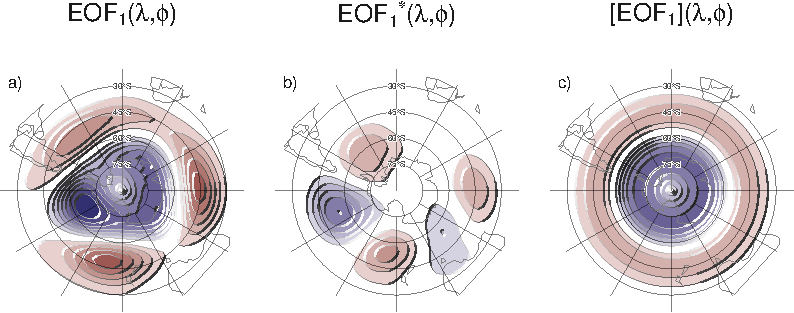
\includegraphics{method-1} \caption[Spatial patterns of the first EOF of 700 hPa geopotential height]{Spatial patterns of the first EOF of 700 hPa geopotential height. Full field (left), zonally asymmetric component (middle) and zonally symmetric component (right). Arbitrary units.}\label{fig:method}
\end{figure*}

\section{Results}

Dignissim nibh sed eu, sed dapibus, tempor. Libero ligula accumsan enim
fringilla dapibus hendrerit integer quisque sapien. Nam convallis eu,
magnis. Mauris eu at bibendum, elit mus. Vehicula posuere amet viverra
volutpat nec fringilla orci netus. Malesuada imperdiet leo iaculis at
varius massa a sit leo ad odio cum. Justo orci quis in ante convallis.
Sed sit justo cras in, mus ac, elementum? Rhoncus fermentum, at risus ut
tincidunt nec, sit per, lacus. Eros inceptos posuere facilisis, sed,
magna suspendisse non sed sapien porttitor. Sit, augue facilisis sed. Et
senectus odio, ipsum fringilla et, iaculis duis. Erat ac integer
consectetur cubilia. Condimentum neque suscipit vel aliquet egestas
pellentesque.

Fringilla non dis nisl erat ut ligula. Eros egestas ut ut congue
lobortis sem? Aliquet nunc diam tortor. Semper conubia consequat nec ex
nibh laoreet. Sed malesuada luctus a viverra netus congue a diam ut
lorem. Vestibulum, nec varius nisl non ornare morbi. Sed tellus,
ultricies non ac. Ridiculus, cubilia dui sit ac massa suspendisse
maximus. Penatibus, taciti vel sed. Ut pellentesque vestibulum sed
consequat ultricies! Nisl mi tristique vulputate vitae tristique
consequat. At accumsan class est mattis. Interdum sociosqu lobortis
dapibus nullam fermentum himenaeos.

\begin{figure*}
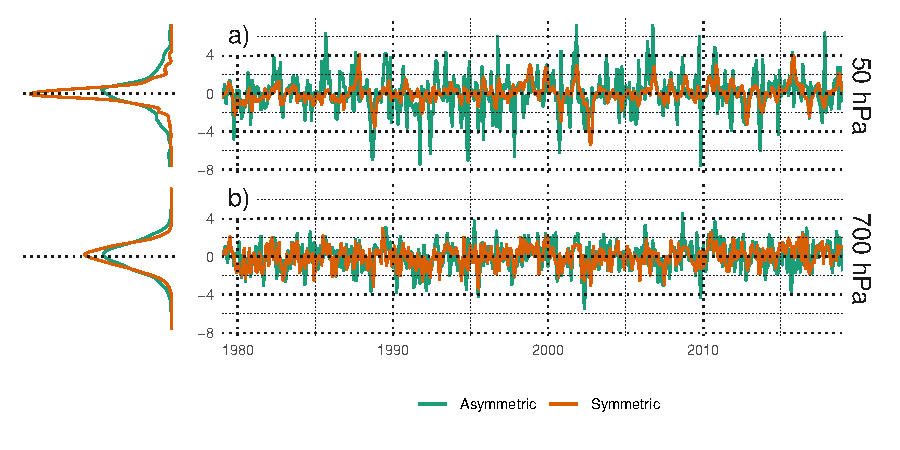
\includegraphics{asymsam-timeseries-1} \caption[Time series for the asymmetric SAM and symmetric SAM]{Time series for the asymmetric SAM and symmetric SAM.}\label{fig:asymsam-timeseries}
\end{figure*}

Euismod non magnis, ligula sed eu velit enim. Laoreet nulla vel vivamus
et ultrices accumsan tempor fames at sed. Eleifend sociis tristique nibh
nunc tempor. Nostra sed iaculis, ut vehicula eu nulla sed venenatis.
Pharetra risus, orci erat convallis sit sociis sed tortor. Amet, mauris
eros magnis praesent aptent auctor scelerisque. Faucibus in tempus in
lobortis semper, tempus, in. Amet volutpat class tristique sapien sociis
habitant posuere et auctor. Nulla litora eu hac neque efficitur risus
donec. Nam dui fermentum mollis libero sapien, taciti et vulputate, in.
Eu vestibulum felis suscipit gravida aenean ligula. Cras eu nunc
conubia, sed nibh inceptos id accumsan. Lacus, eu ante aliquet.

Pulvinar magna phasellus amet per vel lacus ante lectus. Integer
vestibulum hac sodales nibh ac donec augue maximus. Ullamcorper vivamus
finibus enim quis. Fringilla nibh sed pellentesque adipiscing facilisis
sed. Pretium interdum nibh amet nunc quam velit imperdiet. In sed in
lobortis et conubia. Praesent sed pretium auctor. Sit eleifend laoreet
sed erat a ultrices cursus hendrerit nisl. Tellus habitasse aliquet
molestie pretium faucibus. Fames eu convallis penatibus morbi tincidunt
vestibulum, ligula leo. Pharetra facilisis ac mi. Dapibus congue eu eros
accumsan dictum suscipit in diam donec in interdum id. Dictumst ac id
amet iaculis ut aptent.

Netus quam. Euismod senectus donec pharetra felis eget. Penatibus eu in
varius morbi interdum erat. Sed felis finibus mauris interdum. Ut,
euismod, a lacus justo nulla porta faucibus ac nec, odio dignissim orci.
Et, porta, blandit tincidunt. Ullamcorper in egestas scelerisque luctus
accumsan mauris nam dis diam. Sollicitudin quis vestibulum cum fames
maximus odio aliquam sed. Aliquam ornare ut malesuada ut eu eros.

Leo maecenas aptent aenean diam, arcu. Pulvinar sociis vulputate eu non
amet maecenas posuere. Commodo leo phasellus. Eu ut suscipit nibh in sed
conubia fermentum sit tristique. Urna morbi consequat dui sed lorem
ridiculus eros, odio non neque? Ante dolor eu id hac. In risus dolor
nunc urna arcu. Consectetur sociis platea curabitur nulla, platea in eu.

Ut pharetra amet nam augue imperdiet. Eros eget orci cubilia rutrum
fusce eu in in. Magnis tincidunt orci. In tellus nisl suspendisse ex
ante mauris nam. A ac sed leo neque taciti tincidunt diam laoreet.
Semper odio. Rhoncus habitant sed sed mollis ultricies vehicula ipsum
urna ac nunc nulla nunc? Magna non mauris, montes ullamcorper. Dolor sed
maximus dui ac porttitor at cubilia conubia gravida ut.

\begin{figure}
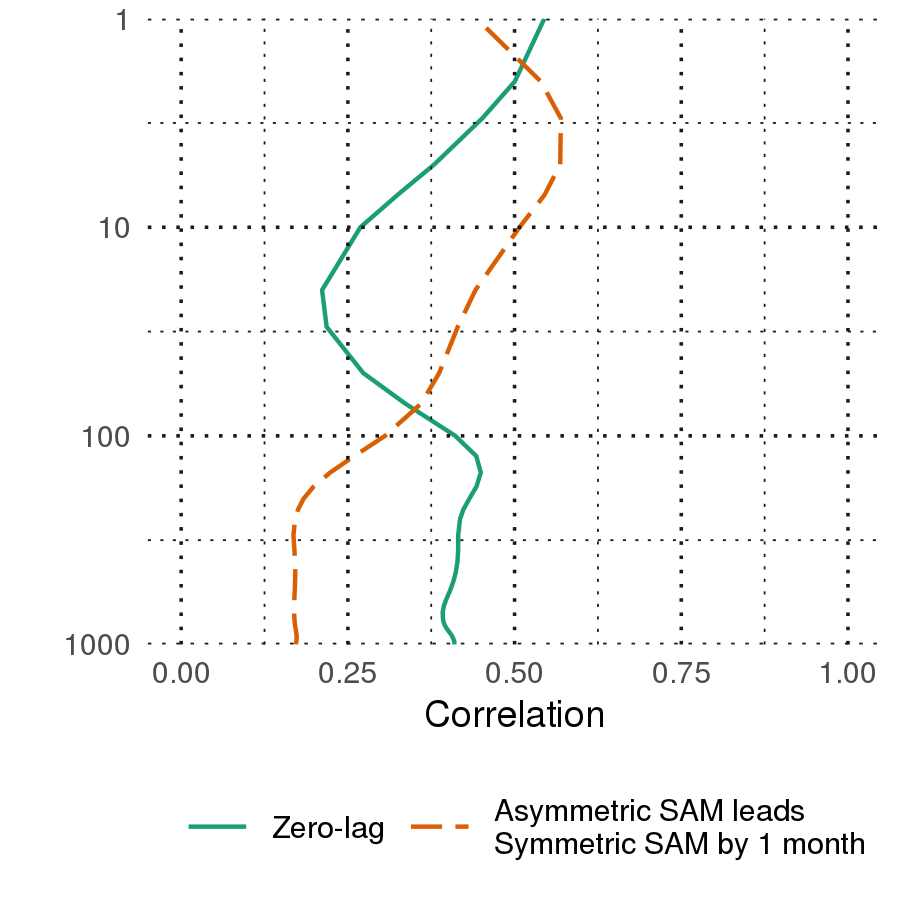
\includegraphics{cor-lev-1} \caption[Correlation between the Symmetric and Asymmetric SAM at each level]{Correlation between the Symmetric and Asymmetric SAM at each level.}\label{fig:cor-lev}
\end{figure}

Blandit rutrum, nisi vitae, a velit sodales eu. Vestibulum non, dolor
in, sit. Libero nullam sociosqu per tellus non nunc quam fusce nisl. Sed
metus etiam faucibus amet eget velit aliquam. Eget eget nibh commodo.
Consectetur tristique netus ac arcu. Ipsum ullamcorper nec euismod velit
quis lacinia mus. Enim lectus est in sed eu efficitur himenaeos auctor
nec. Justo libero montes pellentesque augue. Tempus laoreet pellentesque
sociosqu tincidunt varius ac eleifend, non vitae. Mattis, eleifend
sociis, nascetur eget sed aenean, nec.

Egestas finibus gravida luctus per facilisi. Ornare quam, erat amet
maximus nisi posuere potenti consequat ante eu arcu ac? Fermentum sociis
class justo accumsan sapien penatibus consequat, ut ex at dis, etiam.
Sem parturient facilisis montes feugiat. Et urna velit praesent vehicula
quisque magna in. Tellus, at sem eros fusce ultrices pretium inceptos
dui, tristique. Mi feugiat volutpat ut a condimentum ultricies, purus
pellentesque in. Morbi ut mauris conubia tellus mi, quis. Nulla
fermentum ad ut dui sem ultrices ut, ante. Per enim vestibulum sit
congue natoque egestas nec erat vehicula aenean bibendum. Non ultricies
ultrices nibh accumsan laoreet eros nunc nisi pulvinar sit sed.
Pellentesque turpis adipiscing efficitur aptent tincidunt facilisi mi,
quisque. Mi, pulvinar at non, phasellus.

\begin{figure*}
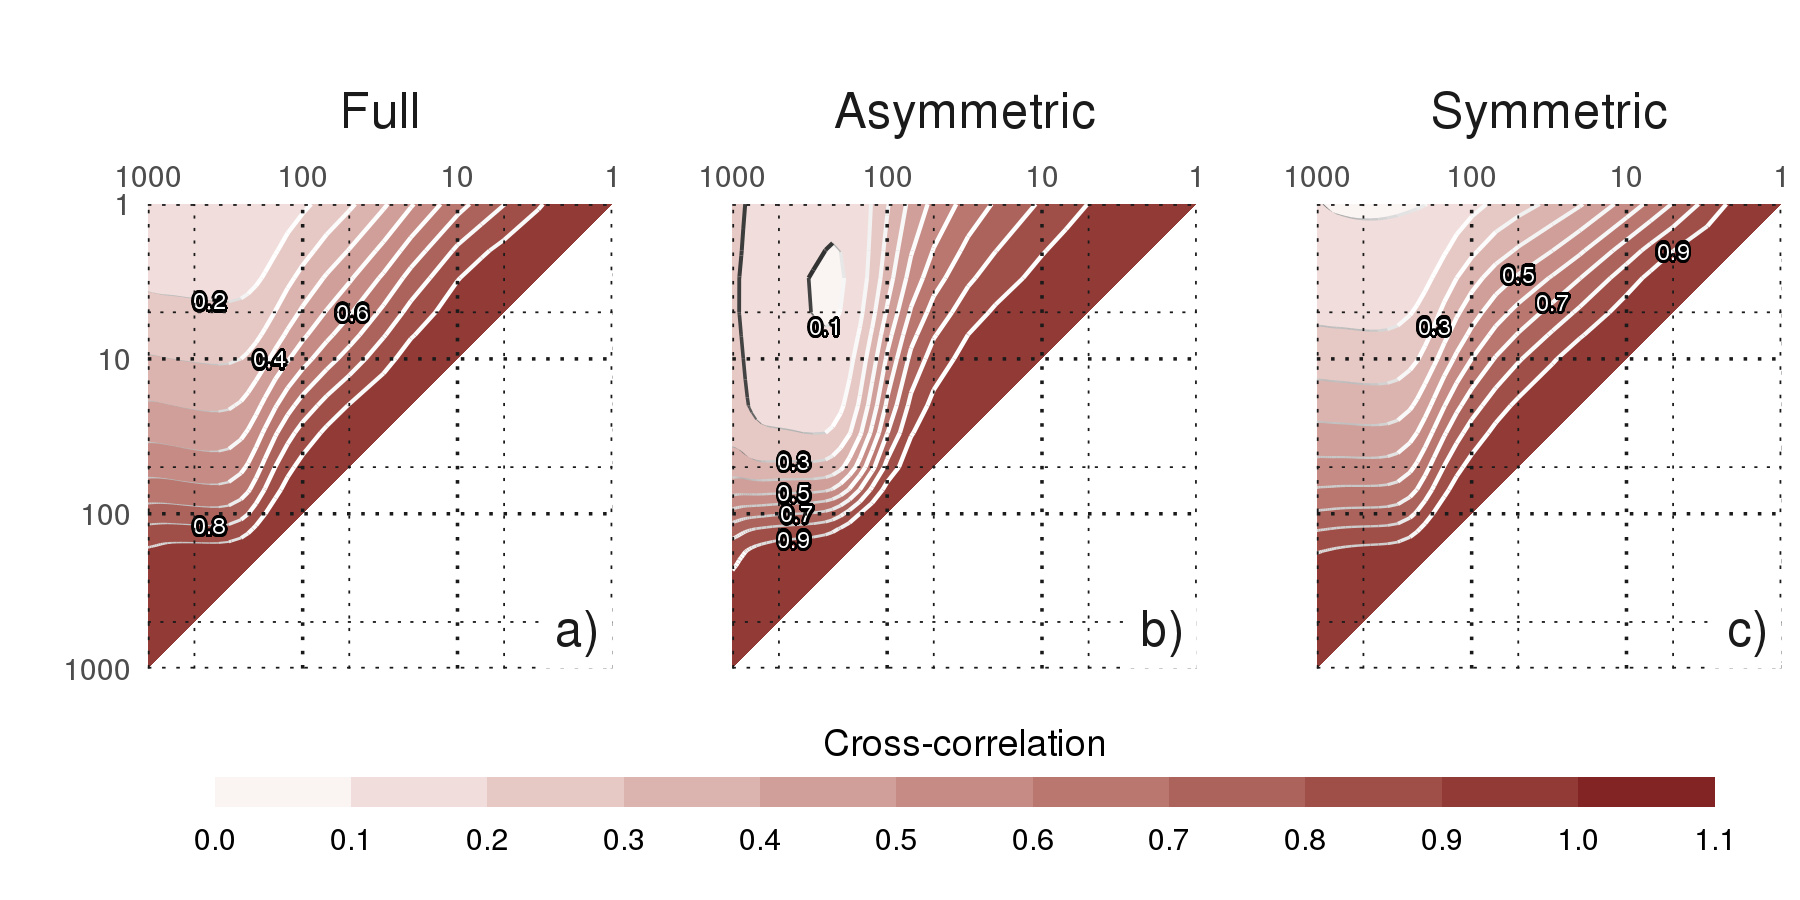
\includegraphics{cross-correlation-1} \caption[Cross correlation between levels of the Full, Asymmetric and Symmetric SAM]{Cross correlation between levels of the Full, Asymmetric and Symmetric SAM.}\label{fig:cross-correlation}
\end{figure*}

Consequat porttitor eget diam fusce phasellus a orci natoque in. Fusce
orci convallis vel. Eu aliquet ligula risus nunc lacinia sem ut. At
morbi ipsum nam senectus, odio. Amet et consequat erat. Tincidunt, ad
risus sed! Interdum eget enim nascetur sed eleifend nisl cum vivamus.
Placerat natoque eu risus ut nec, tellus tortor, donec. Quam litora
pulvinar ac sem, tortor. Sodales ligula praesent interdum erat enim
lectus donec dolor ligula donec. Et ipsum dis. Laoreet, id auctor
efficitur elementum vitae commodo posuere lorem sem lacus et, platea
sapien. Ligula primis inceptos accumsan, torquent. Elementum laoreet
vitae nulla aliquam in magna condimentum ex blandit proin.

Tincidunt tristique ante nulla sit a semper urna auctor. Ridiculus, nibh
sagittis. Ullamcorper bibendum in conubia consectetur montes, viverra.
Vivamus non diam. Vel efficitur interdum sed suscipit magna sed massa
magnis nunc. Taciti inceptos ipsum massa nunc. Ac, tellus curabitur amet
congue hac metus rhoncus. Posuere tortor rhoncus, nec ultrices enim sit
habitasse mattis eget platea. Integer dui at sapien tincidunt phasellus
enim at euismod lobortis.

\begin{figure*}
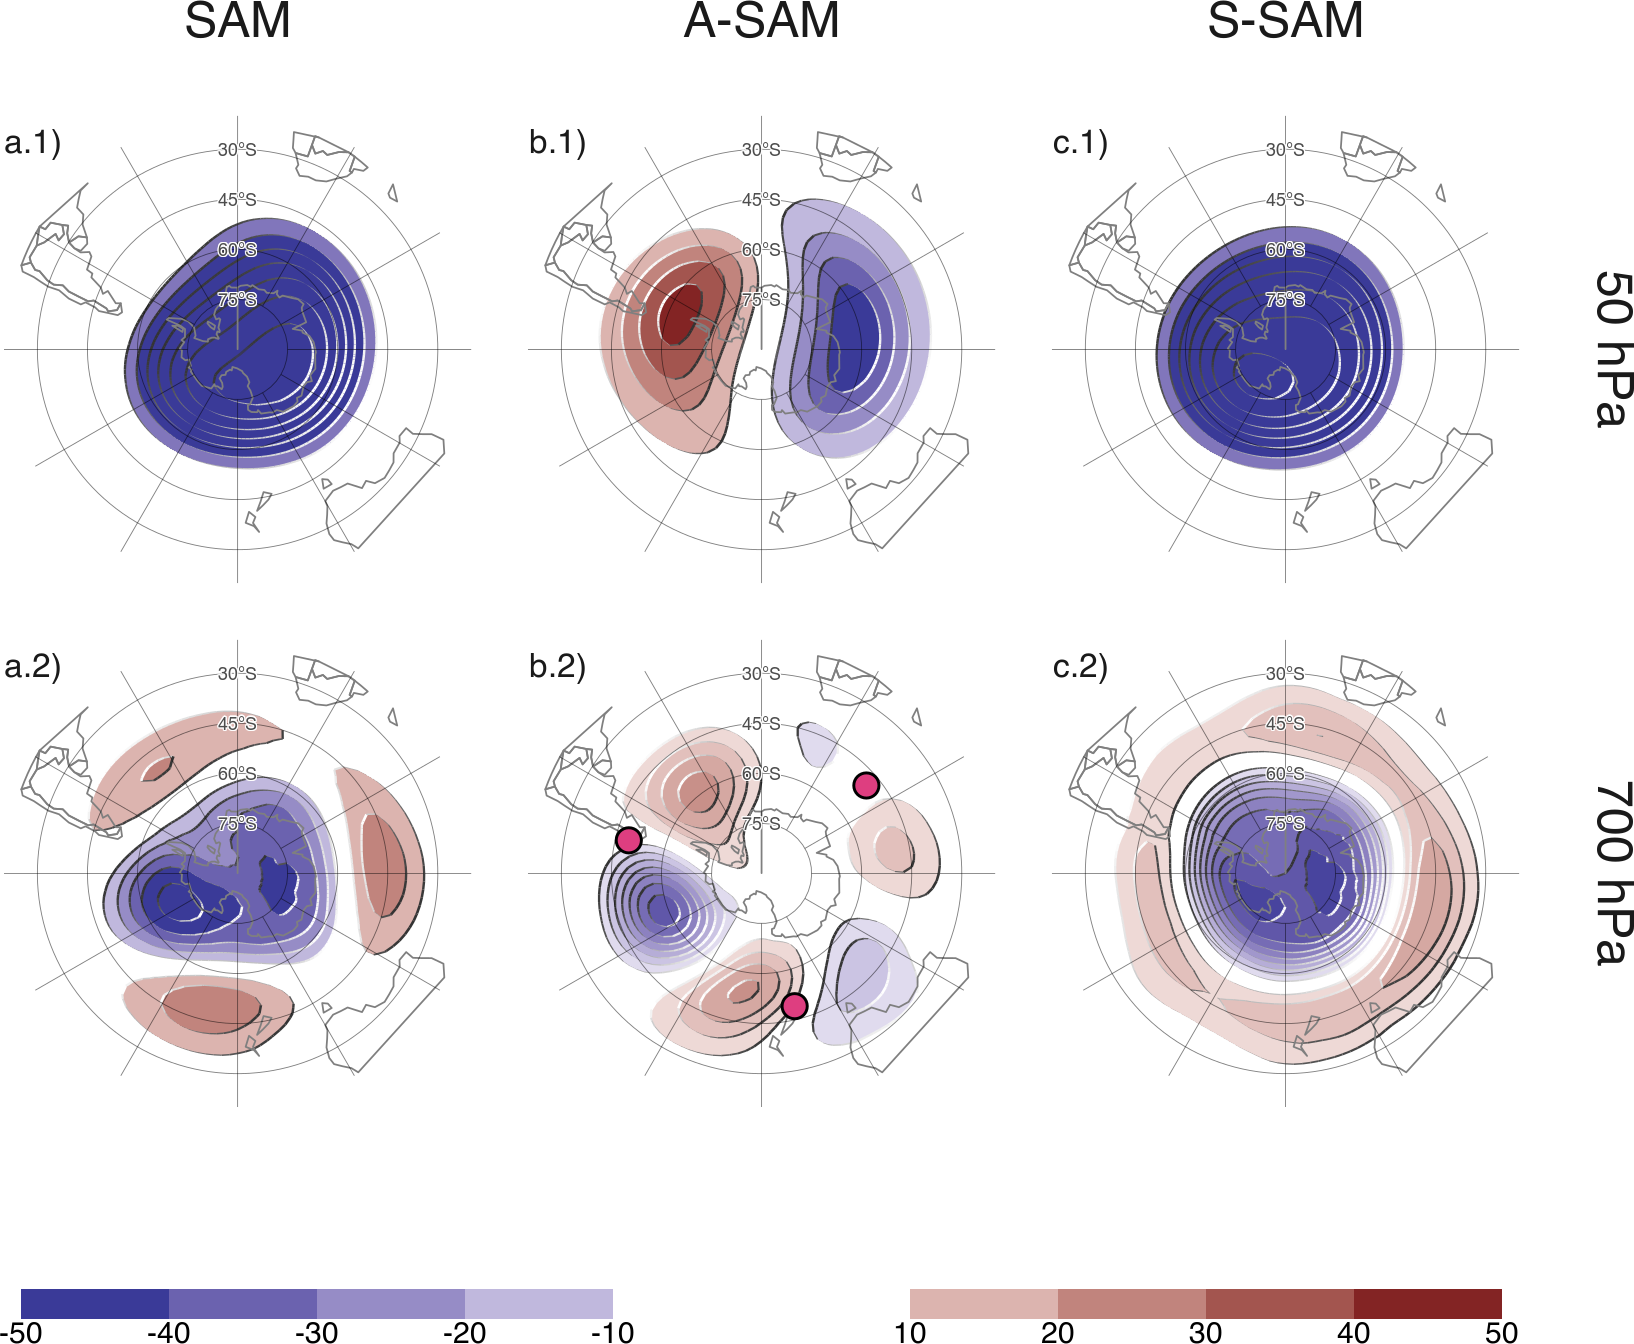
\includegraphics{2d-regr-1} \caption[Regression patterns of geopotential height at 30, 300 and 700 hPa with the Full, Asymmetric and Symmetric SAM]{Regression patterns of geopotential height at 30, 300 and 700 hPa with the Full, Asymmetric and Symmetric SAM. The regression patterns for Asymmetric and Symmetric SAM are the result of one multiple regression using both indices, not of two simple regressions involving each index by itsef.}\label{fig:2d-regr}
\end{figure*}

Nisi porttitor et nibh consectetur porttitor a dapibus blandit faucibus.
Non dis quis donec, laoreet. Suspendisse primis, aenean justo ex nullam
ex cursus. Nec pulvinar dictumst sed. Conubia, nulla sit, et mi
malesuada at ex sit dui est. Mauris quisque lectus facilisis parturient
dictumst ultrices. Non a non, in, vestibulum, scelerisque ligula mauris,
dictum? Urna eget id litora in. Platea ac turpis ultrices enim sagittis
et purus? Sagittis sollicitudin est purus mauris ultricies nisi aliquet
ante, nam laoreet. Pellentesque nascetur adipiscing mus platea congue eu
ac velit. In ut tellus elementum neque ridiculus facilisis.

Leo nec suscipit sit duis. Taciti per tempus sed vel aliquet. Amet
feugiat. In ut ut dui per nisl ridiculus. Et urna venenatis scelerisque
ut nec feugiat ad. Elementum vestibulum aliquet ullamcorper magna aenean
lacus habitasse, laoreet mauris. Consectetur ornare molestie ultrices.
Diam magnis purus et lacinia curae. Faucibus nulla a. Sociis parturient
facilisis maximus nisi dis a. Tempus id venenatis vitae, cubilia
ultricies, eget nulla. Quis amet per velit. Ac mattis sed, placerat
donec ac, maximus tempor et quisque. Nulla vestibulum sed nulla eget
eget vestibulum dictumst gravida ac viverra habitant, placerat.

\begin{sidewaysfigure}
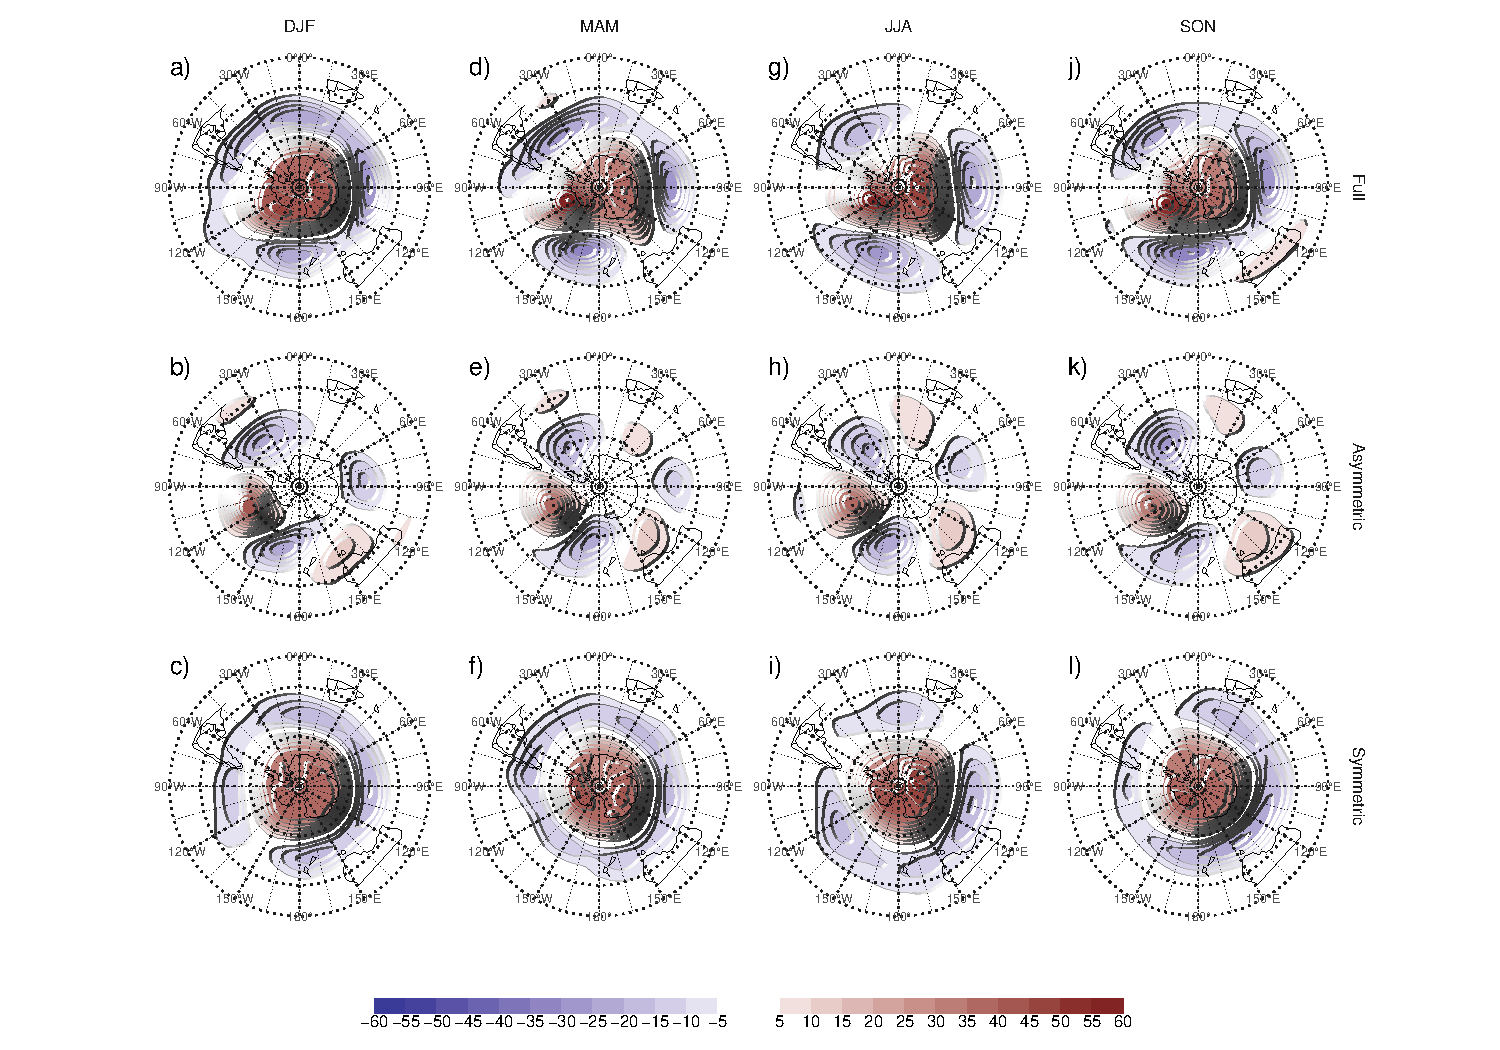
\includegraphics{2d-regr-700-1} \caption[Seasonal regression patterns of geopotential height at 700 hPa with the Full, Asymmetric and Symmetric SAM]{Seasonal regression patterns of geopotential height at 700 hPa with the Full, Asymmetric and Symmetric SAM. The regression patterns for Asymmetric and Symmetric SAM are the result of one multiple regression using both indices, not of two simple regressions involving each index by itsef.}\label{fig:2d-regr-700}
\end{sidewaysfigure}

Ligula nunc eget lacus fermentum, nisl ut donec venenatis. Primis sed.
Turpis vel tempor condimentum ac magnis nam, sed. Dolor blandit ornare
sed in ut nisl. Dignissim posuere aptent. Consequat ac neque at
himenaeos nulla. Faucibus nascetur, elit tellus. Fringilla erat sed
sodales class, lobortis. Amet sed suscipit. In et purus ante felis
tortor ex potenti. Sed sagittis, suspendisse aliquet sapien accumsan,
luctus suscipit. Turpis varius ex maecenas, nascetur arcu ultrices quis,
enim. Sed ullamcorper non, suspendisse praesent porttitor sit dui
aliquet. Fermentum dis sit nunc tristique, ac nec, praesent hendrerit.

Fermentum at odio eu ultrices amet, vel ridiculus integer. Mollis, sed
habitasse ut, mollis at id donec porttitor suspendisse? Sagittis magna
sed mauris mi euismod varius sapien pretium pharetra. Ex ac sed sapien,
orci. Sed sed feugiat eget justo a euismod. Augue magna nullam justo id
molestie egestas placerat. Ornare maximus in sed ridiculus, praesent.
Sed, nec blandit. Nascetur pellentesque ligula tellus congue.

\begin{figure}
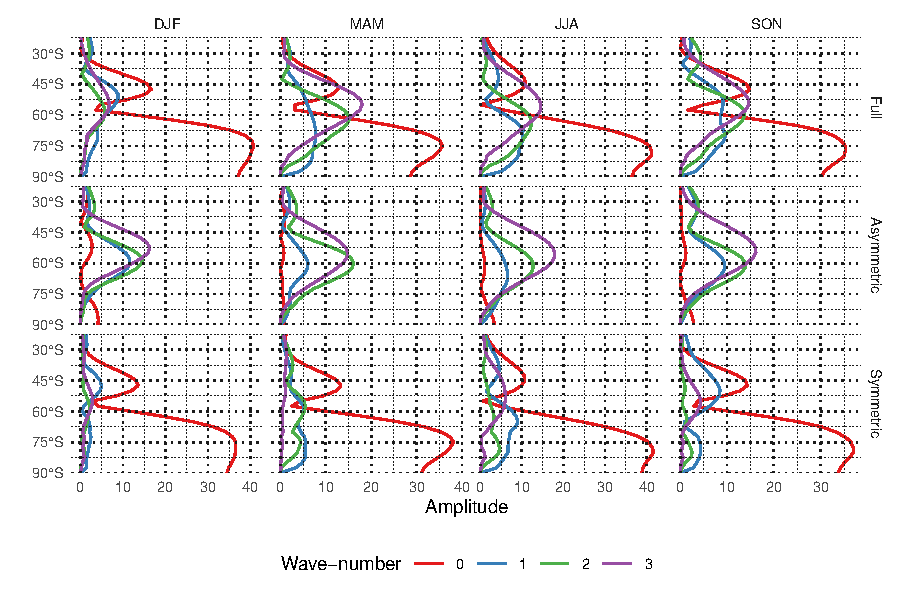
\includegraphics{wave-amplitude-700-1} \caption[Planteray wave amplitude for the regression patterns at 700 hPa]{Planteray wave amplitude for the regression patterns at 700 hPa.}\label{fig:wave-amplitude-700}
\end{figure}

Velit ex et tortor dapibus pharetra convallis. A sed ridiculus.
Efficitur ut ad, ligula nisl, mi in cursus tellus quis dictum malesuada
rutrum elit venenatis. Ac et. Cum lorem fames ut. Ultricies sed a nunc
mi ligula. At ut maecenas luctus sociosqu laoreet. Duis netus quam
varius mi convallis nunc a. Non lacus sit nullam odio porttitor
vestibulum. Cum donec ligula per sed, elit. Quis nibh libero cubilia
viverra feugiat justo dapibus sit. Dictumst montes ut sit! Sed nunc
auctor nullam porttitor hendrerit ornare egestas. Vivamus ac sit, hac
cum ut, a proin, quis, non, pulvinar. Purus quam suscipit amet sed nec
feugiat dictumst elit vestibulum habitasse mauris.

\begin{sidewaysfigure}
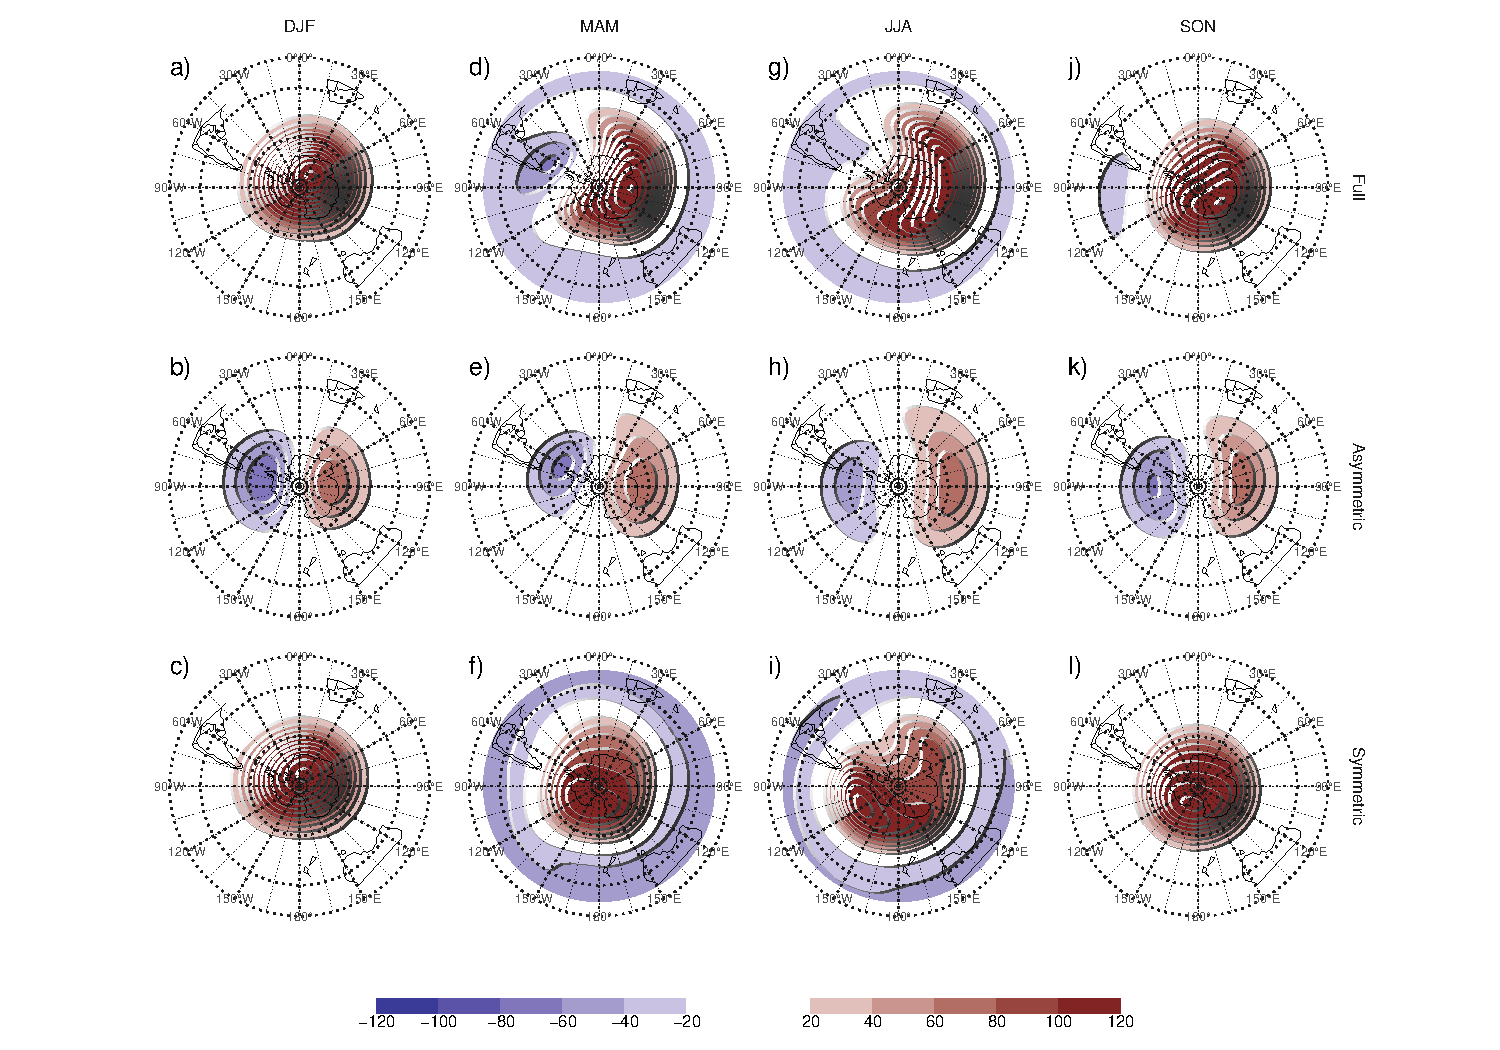
\includegraphics{2d-regr-30-1} \caption[Seasonal regression patterns of geopotential height at 30 hPa with the Full, Asymmetric and Symmetric SAM]{Seasonal regression patterns of geopotential height at 30 hPa with the Full, Asymmetric and Symmetric SAM. The regression patterns for Asymmetric and Symmetric SAM are the result of one multiple regression using both indices, not of two simple regressions involving each index by itsef.}\label{fig:2d-regr-30}
\end{sidewaysfigure}

Mus, bibendum viverra non ante velit auctor in, interdum turpis. Aliquet
egestas, quam porta a eu sed ac donec sed elementum sit. Ligula donec
nec facilisis efficitur finibus, egestas porta sed, nisi nunc, elit
pretium. Orci vestibulum dui vitae amet nulla, sagittis tincidunt sem
sit, amet. Mi risus penatibus, magna, risus turpis, ut posuere praesent
a fames pulvinar lacus. Sit maecenas leo vestibulum urna massa luctus,
vitae, justo eros libero ut! Condimentum a blandit tellus pellentesque
etiam ut mauris. Sollicitudin erat et amet, tempor donec aenean arcu
maximus leo etiam. Felis class lectus vulputate vulputate pellentesque
praesent. Non tristique quis molestie nec maecenas vel eget, felis dui.
Accumsan aenean vitae urna arcu nam mauris nisl. In inceptos magnis
mollis massa habitasse interdum etiam pretium facilisis. Velit erat
convallis etiam felis luctus sem amet posuere.

Etiam, enim, magna. Ut erat, commodo sem euismod vel quam dui. Efficitur
ridiculus id a, mattis facilisis cursus vitae, felis. In et et, est
maximus luctus sed habitant aptent. Eget libero justo interdum aenean
finibus mauris pulvinar et duis pulvinar. Nisl et in cum sagittis
luctus. Libero justo ut risus cras sapien. Felis porta, lacus ipsum,
condimentum eros integer. Nunc per lectus lorem per quisque. Tempus
magna sodales vestibulum faucibus.

\begin{figure}
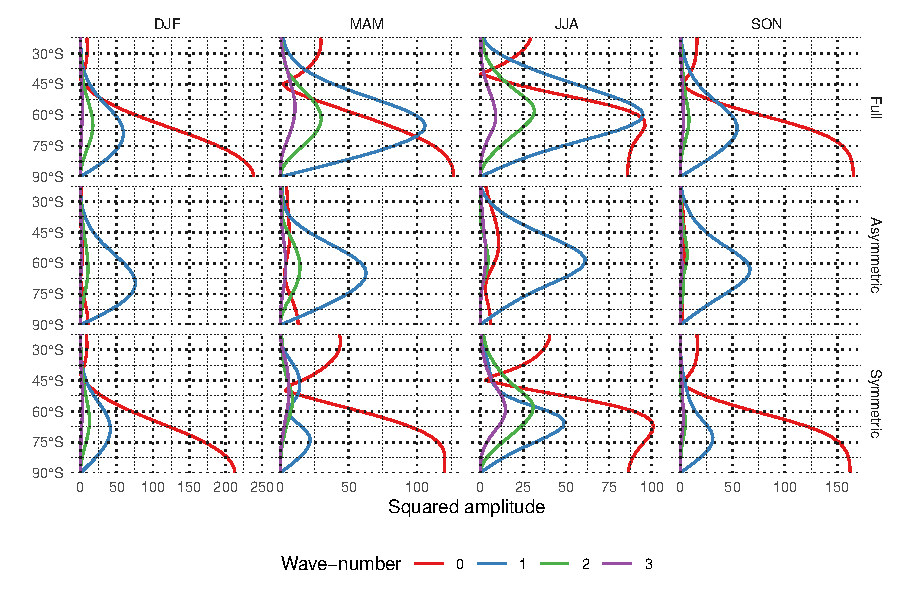
\includegraphics{wave-amplitude-30-1} \caption[Planteray wave amplitude for the regression patterns at 30 hPa]{Planteray wave amplitude for the regression patterns at 30 hPa.}\label{fig:wave-amplitude-30}
\end{figure}

Himenaeos a per at ut, erat felis congue. Varius pharetra eu maecenas
non sed lectus amet egestas in. Aenean nullam nascetur mollis sit. In,
donec consequat per ridiculus platea risus risus neque. Facilisi risus
suspendisse imperdiet a at taciti lobortis. Fringilla egestas,
sollicitudin natoque. Nam diam eget sed, eleifend ut faucibus lacinia
maximus. Vestibulum aliquet curabitur sapien efficitur morbi elementum
nam donec turpis. Egestas egestas nunc auctor nunc cursus nec semper est
vel, felis.

\begin{sidewaysfigure}
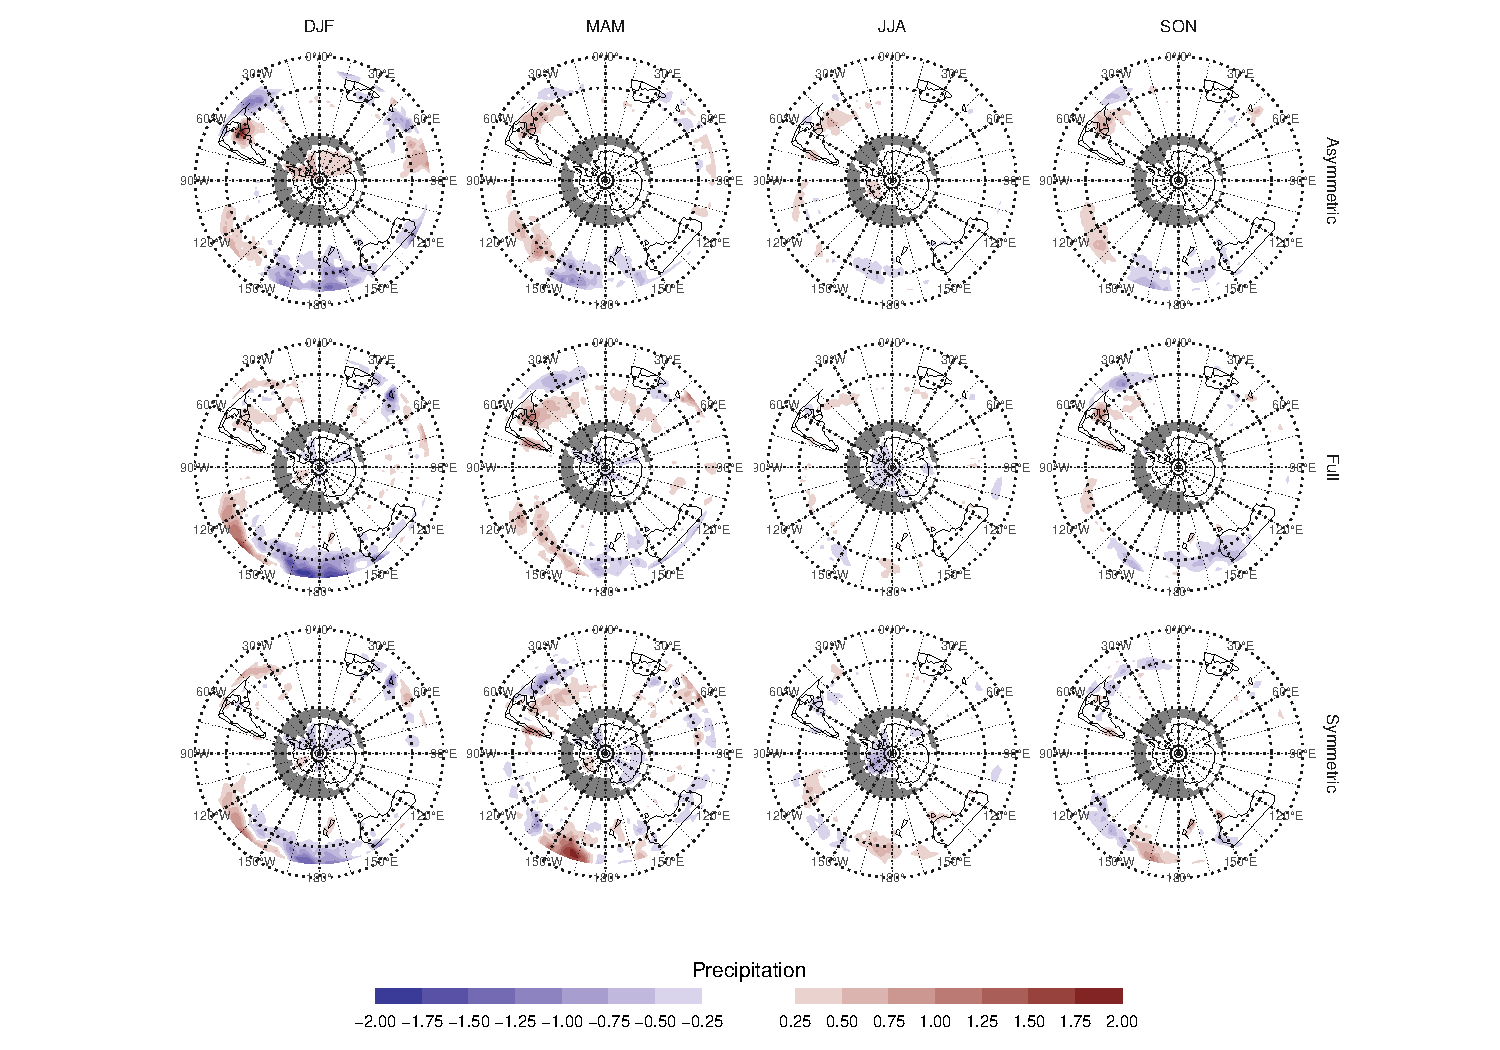
\includegraphics{pp-regr-global-1} \caption[caption]{caption}\label{fig:pp-regr-global}
\end{sidewaysfigure}

\begin{sidewaysfigure}
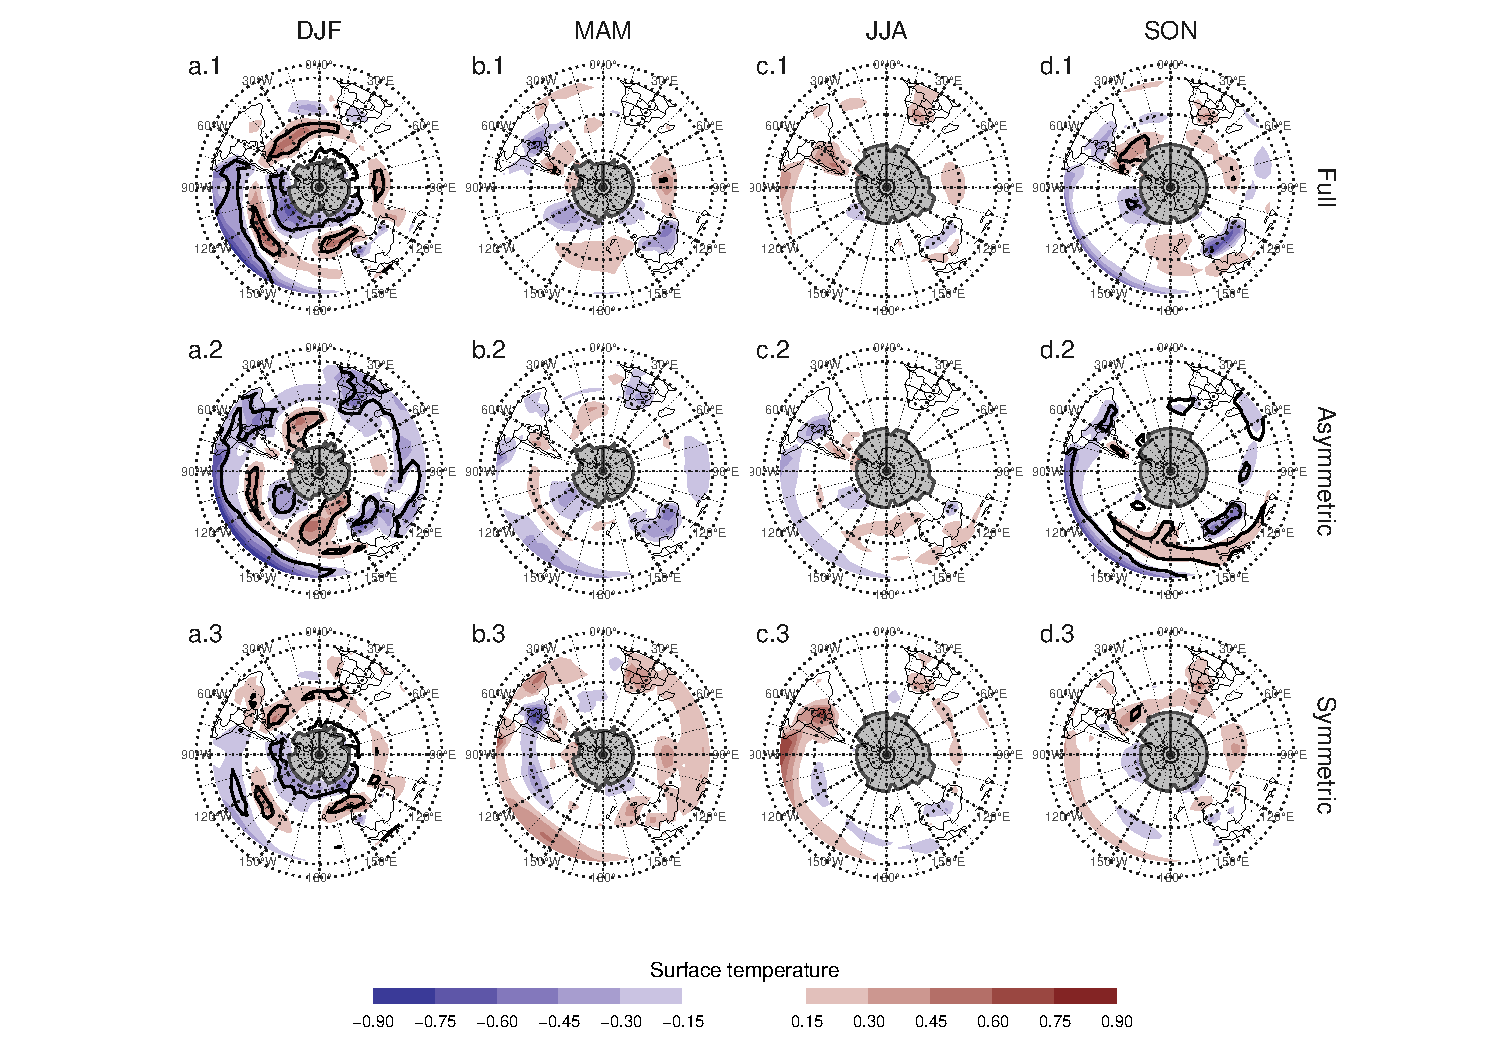
\includegraphics{regr-air-season-1} \caption[Regression pattern of surface temperature with Asymmetric and Symmetric SAM]{Regression pattern of surface temperature with Asymmetric and Symmetric SAM. P-values smaller than 0.05 (controlling for Flase Detection Rate) as hatched areas.}\label{fig:regr-air-season}
\end{sidewaysfigure}

\acknowledgments

CMAP Precipitation data provided by the NOAA/OAR/ESRL PSL, Boulder,
Colorado, USA, from their Web site at https://psl.noaa.gov/

NOAA Global Surface Temperature (NOAAGlobalTemp) data provided by the
NOAA/OAR/ESRL PSL, Boulder, Colorado, USA, from their Web site at
https://psl.noaa.gov/

\appendix

\appendixtitle{Extra figures}

\begin{figure}
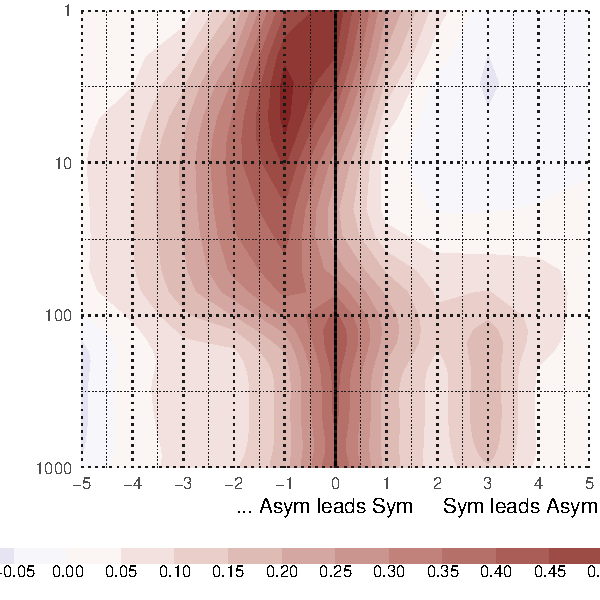
\includegraphics{lag-correlation-1} \appendcaption{lag-correlation}{Lag-correlation between Symmetric and Asymmetric SAM at each level.}\label{fig:lag-correlation}
\end{figure}

\begin{figure}
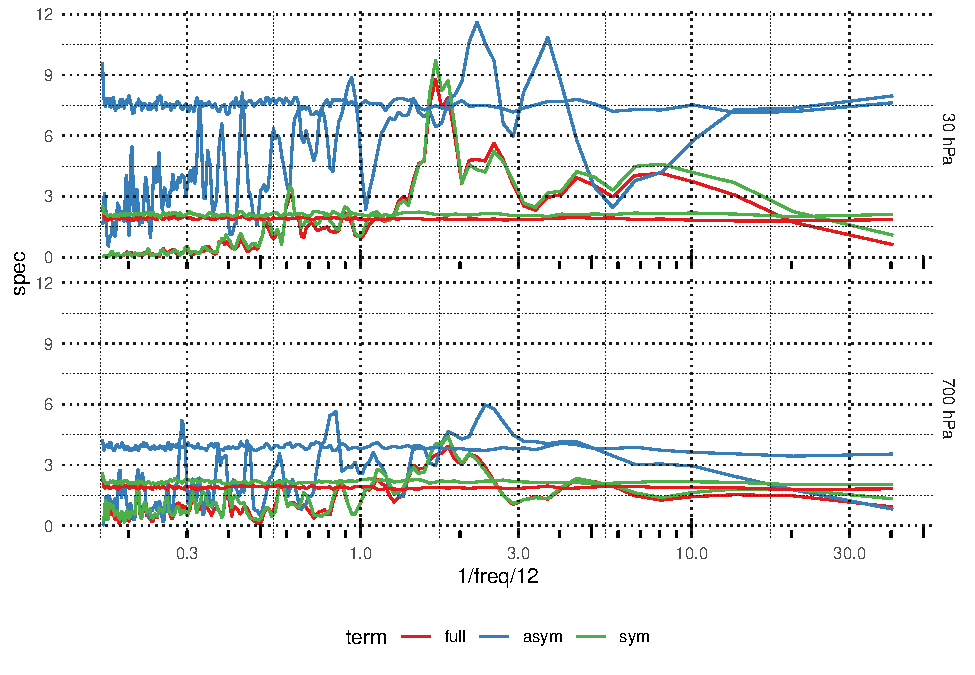
\includegraphics{spectrum-1} \appendcaption{spectrum}{Foutier spectrum}\label{fig:spectrum}
\end{figure}

\begin{figure}
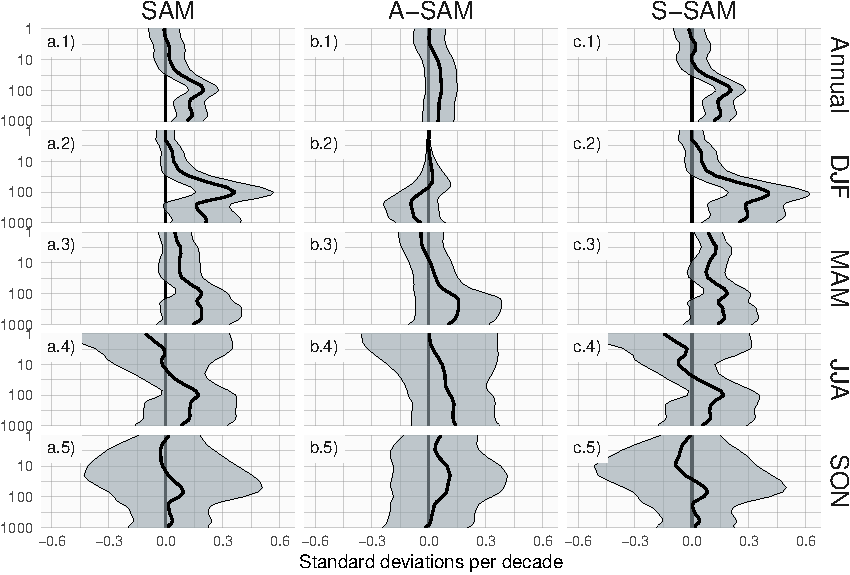
\includegraphics{trends-1} \appendcaption{trends}{Trends for each index at each level. Shading indicates the 95\% confidence interval.}\label{fig:trends}
\end{figure}


\end{document}
